\documentclass[11pt]{article}
% ------------------------------------------------------------------------------------------------
% Affording Generative AI -- English manuscript (compile: pdflatex, bibtex, pdflatex, pdflatex)
% All numbers in tables are generated by code/40_tables_tex.py from the replication package.
% ------------------------------------------------------------------------------------------------
\usepackage[a4paper,margin=1in]{geometry}
\usepackage[T1]{fontenc}
\usepackage[utf8]{inputenc}
\usepackage{mathptmx}
\usepackage{amsmath,amsthm}
\usepackage{booktabs,threeparttable,tabularx,array,multirow}
\usepackage{graphicx}
\usepackage[labelfont=bf,font=small,skip=4pt]{caption}
\usepackage{setspace}
\usepackage[authoryear,round]{natbib}
\usepackage{xcolor}
\usepackage{tikz}
\usetikzlibrary{arrows.meta,positioning,fit,backgrounds}
\usepackage{enumitem}
\usepackage[hidelinks]{hyperref}
\usepackage{xurl}
\urlstyle{same}  % URLs in the text font (no bitmap typewriter fonts)
\setstretch{1.2}
\setlist{itemsep=2pt,topsep=4pt}
\setlength{\emergencystretch}{2em}
\newtheorem{proposition}{Proposition}
\newtheorem{corollary}{Corollary}
\theoremstyle{definition}
\newtheorem{definition}{Definition}
\theoremstyle{remark}
\newtheorem{remark}{Remark}
\newcommand{\AAB}{\mathit{AAB}}
\makeatletter\newcommand{\tabinput}[1]{\@@input #1 }\makeatother % primitive input: safe inside tabular
\definecolor{inkblue}{HTML}{2A78D6}
\definecolor{inkorange}{HTML}{EB6834}
\definecolor{inkgray}{HTML}{52514E}

\title{\textbf{Affording Generative AI:\\ Uniform Prices, Unequal Burdens, and the Two Margins of AI Diffusion}}
\author{TaeHwan Oh\thanks{Independent researcher, Paju, Republic of Korea. ORCID: \url{https://orcid.org/0009-0004-4111-4802}.\newline E-mail: \href{mailto:noah.taehwan@gmail.com}{noah.taehwan@gmail.com}. Data and code: \url{https://doi.org/10.5281/zenodo.23006366} (replication package described in Appendix~\ref{app:data}). This version: 28~September 2026. Comments welcome.}}
\date{Working paper --- September 2026}

\begin{document}
\maketitle

\begin{abstract}
\noindent Consumer generative AI is sold on a price ladder (roughly \$8, \$20, \$100 and \$200 a month) that is nearly identical across countries. I document what this ladder costs relative to income in 201 economies, audit tax-inclusive local App Store prices for ChatGPT, Claude and Gemini in 170 storefronts, and relate burdens to two independent measures of diffusion. Local dollar prices barely respond to income: the elasticity is 0.03--0.04 for \$20 plans and 0.14 for ChatGPT Go, OpenAI's entry tier, compared with 0.23 under purchasing-power-indexed pricing. A \$20 plan therefore costs 0.65\% of per-capita income a year in the median high-income economy and 29\% in the median low-income economy, and 60\% of the covered economies' working-age population lives where it exceeds the 2\% affordability benchmark for broadband. The income elasticity of any generative-AI use is 0.37, about half of which mirrors the income gradient in internet use, and the ratio of AI users to internet users is flat across middle- and low-income groups. Per-capita use of a frontier assistant (Claude; free and paid accounts pooled) rises twice as steeply with income (0.71), and its measured gradient steepened between August 2025 and February 2026. A two-tier adoption model, in which free tiers relax the budget constraint on whether people use AI but not on how much frontier capability they use, is consistent with this contrast, although cross-country data cannot identify price effects. Because exposure and access are both income-graded, larger conditional gains for less-skilled users need not produce cross-country convergence.

\medskip
\noindent\textbf{Keywords:} generative AI; affordability; digital divide; international price discrimination; technology diffusion; development.\\
\noindent\textbf{JEL codes:} O33, O15, L11, L86, D63, F63.
\end{abstract}

\newpage
% ================================================================================================
\section{Introduction}\label{sec:intro}

Much of the field evidence suggests that generative AI helps less skilled and less experienced workers most. Customer-support agents given an AI assistant resolved 15\% more issues per hour, with the largest gains for the least experienced \citep{brynjolfsson2025generative}. Professionals writing with ChatGPT took 40\% less time, and inequality between workers fell \citep{noy2023experimental}. Below-median consultants gained most from GPT-4 inside its capability frontier \citep{dellacqua2023navigating}, and developers with an AI pair programmer completed a task 55.8\% faster \citep{peng2023impact}. If a technology raises the productivity of the less skilled by more, it seems natural to expect it to narrow gaps between workers and, perhaps, between countries.

That expectation assumes that people can use the technology. Whether AI narrows or widens gaps across the world depends on who can use it, how intensively, and at what level of capability. Unlike most earlier general-purpose technologies \citep{bresnahan1995general}, frontier AI capability is sold directly to individuals as a subscription, and the menu of plans is standardised. As of September 2026 the three leading consumer assistants (OpenAI's ChatGPT, Anthropic's Claude and Google's Gemini) all offer a free tier, a standard tier at \$20 and high-usage tiers at about \$100 and \$200 a month, and OpenAI and Google add an entry tier at \$5--8. The upper tiers are distinguished mainly by usage allowances rather than by features (Table~\ref{tab:ladder}). The same dollar price weighs very differently across countries: \$20 a month is 0.3\% of per-capita income in the United States and more than 40\% in Mozambique.

This paper asks what that price structure implies for access and for the distribution of AI's productivity gains, and it separates what current public data can and cannot show. I make four contributions.

First, I measure the \emph{AI affordability burden}, the annual cost of a plan as a share of per-capita income, for 201 economies using 2025 national income, the income classification in force since July 2026, household income shares by quintile, and the affordability benchmark that the United Nations Broadband Commission and the International Telecommunication Union apply to broadband \citep{itu2025ff}. Second, I assemble what is, to my knowledge, the first cross-country audit of local AI subscription prices: tax-inclusive prices listed for nine plans of the three assistants in every Apple App Store storefront (218 codes, 170 with local price lists), collected on a single day from a single payment channel. Third, I relate burdens to two independent, public measures of diffusion that capture different margins: Microsoft's AI User Share \citep{misra2025measuring,microsoft2026q2}, the share of the working-age population that used any generative-AI product, and Anthropic's AI Usage Index \citep{appel2025uneven,anthropic2026aei}, per-capita use of a frontier assistant. In doing so I document that 36 of the 147 economies in the Microsoft data, including 20 of the 23 low-income economies, are regional averages rather than country estimates, which bears on any claim about the poorest countries. Fourth, I develop a simple model that organises the evidence and delivers three testable or quantifiable propositions.

The findings can be summarised as five facts. \emph{Prices are nearly uniform.} Across storefronts the income elasticity of local dollar prices is 0.03--0.04 for the \$20 tiers and 0.14 for ChatGPT Go, OpenAI's entry tier (0.03 for Google's AI Plus). Indexing prices to local price levels would imply an elasticity of 0.23. Every App Store storefront in a low-income economy prices in U.S. dollars, and 36\% of low-income economies have no local storefront at all. \emph{Burdens are therefore steeply income-graded.} A \$20 plan costs 0.65\% of per-capita income a year in the median high-income economy, 3.1\% in upper-middle-, 8.7\% in lower-middle- and 29\% in low-income economies. It meets the 2\% benchmark only where per-capita income is at least \$12,000 (roughly the high-income threshold), and 60\% of the working-age population in the economies covered lives where it does not. Even for the richest fifth of households in the median low-income economy, one plan would cost 13\% of average income. \emph{The extensive margin is only moderately income-graded.} The income elasticity of the AI User Share is 0.37 on country-specific estimates. In an accounting sense about half of it mirrors the income gradient in internet use, and the ratio of AI users to internet users is essentially flat, at about 23\%, across upper-middle-, lower-middle- and low-income groups. Conditional on income, however, differences in internet use are not associated with AI use, so the split is not a causal share. The dispersion of adoption is falling in logs but rising in percentage points: the gap between the median high-income and lower-middle-income economy widened from 16.3 to 20.3 points between the first half of 2025 and the second quarter of 2026. \emph{The intensive, frontier margin is twice as income-graded.} On the 96 economies covered by both measures, of which only one (Rwanda) is low-income, the income elasticity of per-capita Claude use is 0.71 against 0.37 for any use (difference 0.34; bootstrap 95\% interval 0.27--0.40). The gap survives a log-odds transformation, the exclusion of high-income economies, controls for connectivity and education, and earlier measurement windows. Because the index pools the free and paid accounts of one vendor, it proxies the frontier margin only imperfectly. On a common sample the measured elasticity rose from 0.68 in August 2025 to 0.74 in February 2026, a period in which the index's product coverage also changed, and has been stable since. \emph{Aggregate implications are modest in levels but unequal in ratios.} Illustrative Hulten-style calculations, in which occupational exposure and population-wide use stand in for the task exposure and within-task adoption that the formula requires, imply output gains of about 1.2\% of GDP in high-income and 0.1\% in low-income economies for a 20\% task-level productivity gain, an eleven-fold ratio driven jointly by exposure and adoption.

A two-tier adoption model offers one explanation for why the margins differ. In the model, when a free tier exists, the decision to use AI at all is governed by non-monetary hurdles (connectivity, skills, language), so the price of the paid tier drops out of the extensive margin. Buying more capability, by contrast, depends on the ratio of price to income, which inherits the full income gradient unless prices are localised. The model predicts a steeper income gradient on the frontier margin whenever the price hurdle exceeds the non-price hurdle and localisation is weak, which is consistent with the data. A second proposition shows that larger conditional gains for less-productive users are neither necessary nor sufficient for convergence. As proxies for task exposure and adoption I use the employment shares of exposed occupations, 34\% and 11\% in high- and low-income economies \citep{gmyrek2025generative}, and current user shares. On these proxies, low-income adoption would have to reach 100\% for AI to narrow the relative gap if task-level gains were equal, and 50--67\% even if they were 1.5--2 times larger, compared with about 9\% today. A third result translates price burdens into a \emph{capability lag}. Because the API price of any fixed capability level falls by an order of magnitude or more each year \citep{cottier2025llm}, a user who can afford only a fraction of the frontier price would, if such cost declines passed through to consumer tiers, lag the frontier by roughly the log price ratio divided by the rate of price decline. The implied lag would range from a few months to about a year, which is consequential when returns accrue to frontier capability.

This paper relates to several literatures. Studies of who adopts generative AI within countries find adoption skewed toward the young, the educated and higher earners \citep{bick2024rapid,humlum2025unequal}. I show the analogous cross-country gradient and decompose it by margin. Cross-country usage studies based on web traffic, telemetry or conversation data document large gaps by income \citep{liu2024who,liu2025who,misra2025measuring,chatterji2025how,appel2025uneven,daepp2026how,iscenko2026atlas}. I link them to prices and to each other, and I flag a measurement issue in the most widely used series. Earlier cross-country work on computers and the internet found income and human capital to be the main correlates of adoption \citep{caselli2001cross,chinn2007determinants}, and work on mobile telephony in Africa documented the role of prices and networks \citep{aker2010mobile,bjorkegren2019adoption}. The affordability literature for telecommunications \citep{itu2025ff} supplies the benchmark that I extend to AI. The literature on international pricing \citep{goldberg1997goods,cavallo2014currency} and on price discrimination \citep{mussa1978monopoly,varian1985price,aguirre2010monopoly} informs the audit of local prices. Studies of exposure to AI across occupations and countries \citep{felten2021occupational,eloundou2024gpts,pizzinelli2023labor,cazzaniga2024genai,gmyrek2025generative} and of its aggregate effects \citep{acemoglu2025simple,filippucci2024impact} supply the exposure and productivity parameters of my illustrations, and development-oriented assessments \citep{korinek2021artificial,undp2025hdr,unctad2025tir,worldbank2026wdr} frame the policy stakes. Finally, the literature on technology diffusion has long distinguished the timing of adoption from the intensity of use \citep{comin2004cross,comin2010exploration}. \citet{comin2018technology} show that for earlier technologies adoption lags converged across countries while usage intensity diverged. The evidence here suggests that generative AI may be following a similar pattern at an early stage.

The analysis is descriptive. Because a common dollar price makes the burden a monotone transformation of income, a cross-country association between burdens and use cannot identify a price effect. I therefore use the model to derive predictions that distinguish margins, and I set out the quasi-experimental designs that the rapid rollout of localised entry tiers now makes possible. The paper proceeds as follows. Section~\ref{sec:background} describes the price ladder, Section~\ref{sec:model} presents the framework and Section~\ref{sec:data} describes the data. Section~\ref{sec:results} reports results, Section~\ref{sec:discussion} discusses interpretation, policy and limitations, and Section~\ref{sec:conclusion} concludes. Proofs, data construction and additional tables are in the appendices.

% ================================================================================================
\section{Background: the AI price ladder}\label{sec:background}

Table~\ref{tab:ladder} summarises the consumer plans of the three leading assistants as documented on vendors' official pages on 27 September 2026, together with the U.S. App Store price of the same plans. Three features stand out.

\begin{table}[t]
\centering
\begin{threeparttable}
\caption{The consumer price ladder of three leading AI assistants, September 2026}\label{tab:ladder}
\small
\begin{tabularx}{\textwidth}{@{}l>{\raggedright\arraybackslash}X>{\raggedright\arraybackslash}X>{\raggedright\arraybackslash}X@{}}
\toprule
Tier & OpenAI (ChatGPT) & Anthropic (Claude) & Google (Gemini) \\
\midrule
Free & Free & Free & Free \\
Entry & Go: \$8 [\$8.00]; launched in India Aug.\ 2025, 170 further countries, U.S.\ Jan.\ 2026; ads tested & --- & AI Plus: [\$4.99] \\
Standard & Plus: \$20 [\$19.99] & Pro: \$20 monthly, \$17 annual [\$20.00] & AI Pro: [\$19.99] \\
High usage & Pro \$100: 5$\times$ Plus usage [\$100] & Max: ``from \$100'', 5$\times$ or 20$\times$ Pro usage [\$124.99; \$249.99] & AI Ultra \$100: 5$\times$ Pro usage \\
Highest usage & Pro \$200: 20$\times$ Plus usage [\$200]; new sign-ups paused since 10 Sep.\ 2026 & (Max 20$\times$, see above) & AI Ultra \$200 (was \$250): 20$\times$ Pro usage [\$199.99] \\
\bottomrule
\end{tabularx}
\begin{tablenotes}[flushleft]\footnotesize
\item \emph{Notes:} Official U.S. web prices per month, with U.S. App Store prices in brackets (27 September 2026, before sales tax). OpenAI: ``Both Pro tiers include the same core capabilities. The main difference is usage allowance'' \citep{openai2026pro}; Plus price and separate API billing from \citet{openai2026plus}; Go from \citet{openai2026go}. Anthropic: \citet{anthropic2026pricing} (prices exclude tax). Google: new \$100 Ultra tier and \$200 Ultra (down from \$250) announced 19 May 2026 \citep{google2026io}. Google's plan page displays region-dependent prices, so bracketed App Store prices are shown for AI Plus and AI Pro.
\end{tablenotes}
\end{threeparttable}
\end{table}

\emph{Convergence.} The three menus have converged on nearly the same rungs: a free tier, an entry tier, a \$20 standard tier, and tiers at about \$100 and \$200. Using several assistants multiplies the cost: a professional who keeps the \$20 tier of all three assistants pays about \$60 a month, and one who keeps the 5$\times$ tier of all three pays about \$300.

\emph{Quantity, not intelligence.} The upper rungs are differentiated primarily by usage allowances (``5$\times$'' and ``20$\times$'' the standard tier) and, secondarily, by access to the most capable model variants and features. With near-zero marginal cost of replication but non-trivial inference costs, digital goods lend themselves to versioning \citep{goldfarb2019digital}, and the menu is a textbook instance of second-degree price discrimination by quantity and quality \citep{mussa1978monopoly}. The free and entry tiers are deliberately degraded versions of the standard tier: ChatGPT Go, for instance, offers an ``Instant'' model with lower caps, while Plus offers the ``Thinking'' model with higher limits \citep{openai2026go}. A higher price therefore buys more frontier capability per month.

\emph{Localisation happens at the bottom of the ladder.} The entry tiers are the vendors' instrument for reaching lower-income markets: ChatGPT Go launched in India in August 2025 and was rolled out to 170 further countries before its U.S. launch at \$8 in January 2026 \citep{openai2026go}. Section~\ref{sec:prices} shows that OpenAI's entry tier is the only rung whose local price varies materially with income. Promotional give-aways, such as bundles of premium plans with mobile subscriptions in India, further lower effective prices in some markets, but they are temporary and country-specific.

% ================================================================================================
\section{Framework}\label{sec:model}

\subsection{The affordability burden}

\begin{definition}[AI affordability burden]
For a plan with monthly price $p_c$ in country $c$ (current U.S. dollars) and per-capita income $y_c$ (current U.S. dollars),
\begin{equation}
\AAB_c(p_c) = \frac{12\,p_c}{y_c}\times 100 .
\label{eq:aab}
\end{equation}
\end{definition}

The burden is a normalised price: it states how large the price is relative to average income. It is not a budget share and does not measure what anyone spends. The measure follows the convention of the ITU's broadband affordability statistics, which express the monthly price of an entry-level basket as a share of monthly GNI per capita and assess it against the 2\% benchmark of the UN Broadband Commission \citep{itu2025ff}. The benchmark maps into a threshold income: a plan priced at $p$ meets it if and only if $y_c \geq 600\,p$, that is, \$12,000 for a \$20 plan and \$4,800 for an \$8 plan.

Because average income conceals distribution, I also compute burdens at quintile means, approximating the mean income of quintile $q$ by $y_{cq} = y_c\, s_{cq}/0.2$, where $s_{cq}$ is the quintile's survey-based income (or consumption) share. GNI also includes income that does not accrue to households, so I report burdens relative to household final consumption per capita as well.

\begin{remark}[What a PPP denominator measures]\label{rem:ppp}
For a service priced in dollars, the burden relative to income at market exchange rates is the relevant quantity. Dividing the dollar price by income at purchasing-power parity instead yields $12p/y^{PPP}_c = 12\,(p\cdot PLR_c)/y_c$, where $PLR_c = y_c/y^{PPP}_c$, the ratio of Atlas to PPP income, is a proxy for the price level relative to the United States.\footnote{Because the Atlas method averages exchange rates over three years, the ratio differs from the same-year GDP price-level ratio by a median of 3.1\% (90th percentile 8.3\%) across 197 economies. Its income elasticity is 0.228, against 0.224 for the GDP price-level ratio.} It is therefore the burden that would obtain if the vendor indexed its local price to this price-level proxy, $p_c = p\cdot PLR_c$. It describes a counterfactual pricing policy and is not a robustness check on the same quantity. Because the price level rises with income \citep{balassa1964purchasing,samuelson1964theoretical}, and PPP conversion factors are designed for broad consumption baskets rather than internationally priced digital services \citep{deaton2010understanding}, the PPP ratio should be read as the burden under purchasing-power-indexed pricing. Section~\ref{sec:prices} compares actual pricing with this benchmark.
\end{remark}

\subsection{Two margins of access}

The model borrows the standard ingredients of technology-adoption models with heterogeneous returns \citep{suri2011selection,foster2010microeconomics}. Consider individuals $j$ in country $c$ with income $y_j$ and a productivity-value parameter $\theta_j$, so that access to AI of quality $q$ is worth $\theta_j y_j q$ per month. Let $x_j = \ln(\theta_j y_j) \sim N(\mu_c, s^2)$, where $\mu_c$ increases one-for-one with mean log income in the country. A share $\kappa_c$ of the population is online (connectivity and other complements, with $\kappa_c$ increasing in income). A free tier offers quality $q_F$; a paid tier offers $q_P > q_F$ at local price $p_c$. Using the free tier involves a non-monetary cost $\tau$ (time, skills, language). A connected individual uses AI if $\theta_j y_j q_F \geq \tau$ and pays for the frontier tier if $\theta_j y_j (q_P - q_F) \geq p_c$.\footnote{If $p_c/(q_P-q_F) \geq \tau/q_F$, anyone who pays also uses. Heterogeneity in $\tau$ can be absorbed into $\theta_j$.} The \emph{extensive margin} (any use) and the \emph{frontier margin} (paid use) are
\begin{equation}
D_c = \kappa_c\,\Phi(z^D_c),\quad z^D_c = \frac{\mu_c - \ln(\tau/q_F)}{s};\qquad
P_c = \kappa_c\,\Phi(z^P_c),\quad z^P_c = \frac{\mu_c - \ln\big(p_c/(q_P-q_F)\big)}{s}.
\label{eq:margins}
\end{equation}
Let $\beta \equiv \partial\ln p_c/\partial\ln y_c$ denote the elasticity with which the vendor localises its price to income, and let $h(z) = \phi(z)/\Phi(z)$, which is strictly decreasing.

\begin{proposition}[Two margins]\label{prop:margins}
The income elasticities of the two margins are
\[
\varepsilon_D = \varepsilon_\kappa + \frac{h(z^D_c)}{s}, \qquad \varepsilon_P = \varepsilon_\kappa + (1-\beta)\,\frac{h(z^P_c)}{s}.
\]
If the paid hurdle exceeds the free hurdle, $p_c/(q_P-q_F) > \tau/q_F$, and pricing is not localised ($\beta=0$), then $\varepsilon_P > \varepsilon_D$. For given hurdles $(z^D_c, z^P_c)$, the difference falls with $\beta$ and changes sign before $\beta = 1$.
\end{proposition}

The proposition formalises how a free tier changes the role of price in the divide. Price enters only the frontier margin, so a common dollar price steepens that margin's income gradient without affecting the extensive margin, which is governed by connectivity ($\varepsilon_\kappa$) and non-price hurdles. Localisation flattens the frontier margin in proportion to $\beta$. In the data, the Microsoft AI User Share approximates $D_c$. The Anthropic AI Usage Index, per-capita use of a frontier assistant, combines the share of users with their intensity of use and therefore probably weights users of the higher-allowance paid tiers heavily, although it does not identify them. It serves as an imperfect proxy for $P_c$ scaled by intensity. Section~\ref{sec:twomargins} examines whether the data are consistent with $\varepsilon_P > \varepsilon_D$.

\subsection{Access-conditional equalisation}

Let two economies (or groups) $H$ and $L$ have output per worker $y_H > y_L$. Following Hulten's theorem \citep{hulten1978growth} as applied to AI in a task-based framework \citep{acemoglu2019automation,acemoglu2025simple}, AI raises output by $\Delta Y_i/Y_i = s_L E_i a_i g_i$, where $s_L$ is the labour share, $E_i$ the share of labour tasks exposed to AI, $a_i$ the adoption rate in exposed tasks and $g_i$ the task-level productivity gain. The relative gap moves from $R_0 = y_H/y_L$ to
\begin{equation}
\frac{R_1}{R_0} = \frac{1 + s_L E_H a_H g_H}{1 + s_L E_L a_L g_L}.
\label{eq:ratio}
\end{equation}

\begin{proposition}[Access-conditional equalisation]\label{prop:equal}
The relative gap narrows if and only if $E_L a_L g_L > E_H a_H g_H$. Equivalently, the adoption rate in $L$ needed to avoid divergence is
\[
a_L^{*} = a_H \cdot \frac{E_H}{E_L}\cdot \frac{g_H}{g_L}.
\]
Larger conditional gains for the less productive ($g_L > g_H$) are neither necessary nor sufficient for convergence.
\end{proposition}

The result separates two statements that are often conflated. ``AI helps the less skilled more'' is a statement about $g$ conditional on use, whereas ``AI narrows gaps'' also depends on exposure $E$ and adoption $a$. Field evidence on $g$ is itself mixed outside the settings above: in a randomised trial with Kenyan entrepreneurs, access to a GPT-4 business mentor raised the performance of initially high performers by over 15\% and lowered that of low performers by nearly 10\% \citep{otis2025uneven}. I refer to the possibility that AI equalises conditional on use yet widens gaps unconditionally as the \emph{AI access paradox}. Section~\ref{sec:scenarios} quantifies $a_L^*$.

\subsection{A moving frontier: from price gaps to capability lags}

Frontier capability is sold at a roughly constant price $\bar p$ (the \$20 rung has not moved since 2023), while the cost of any fixed level of capability falls quickly: \citet{cottier2025llm} estimate that API inference prices for a given level of performance fall by 9$\times$ to 900$\times$ per year, depending on the capability threshold. Let the price of the capability that was at the frontier at date $t_0$ decline at rate $\delta$, $p(t) = \bar p\, e^{-\delta(t-t_0)}$.

\begin{proposition}[Capability lag]\label{prop:lag}
A user who can spend $b<\bar p$ per month can afford, at any date, the capability that was at the frontier $L$ years earlier, where
\[
L = \frac{\ln(\bar p/b)}{\delta}.
\]
\end{proposition}

With a 2\%-of-income budget, the median low-income economy (per-capita GNI \$830) can spend \$1.38 a month. Relative to \$20, this implies $L$ of 0.4 years at the fastest and 1.2 years at the slowest decline rate. For the median lower-middle-income economy the lag is 0.2--0.7 years, and for the median high-income economy it is zero. These are cost-parity lags. Because $\delta$ is calibrated on API prices while consumers buy discrete subscription tiers (Table~\ref{tab:ladder}), they describe consumer access only insofar as falling costs pass through to the free and entry tiers, for instance when an earlier frontier model moves into a free tier. That pass-through is not measured here. To the extent that it occurs, price barriers are better described as time lags than as permanent exclusion. Open-weight models reinforce the point: they reach similar performance within months of closed frontier releases and have taken a growing share of API token volume \citep{microsoft2026q2,aubakirova2026state,nagle2025latent}. Whether a lag of months has economic consequences depends on whether returns accrue to absolute capability or to capability relative to competitors. In contests such as export markets, software services or research, it plausibly does.

% ================================================================================================
\section{Data}\label{sec:data}

Table~\ref{tab:data} lists sources and coverage, and Appendix~\ref{app:data} describes how the variables are constructed.

\begin{table}[t]
\centering
\begin{threeparttable}
\caption{Data sources}\label{tab:data}
\small
\begin{tabularx}{\textwidth}{@{}>{\raggedright\arraybackslash}p{3.3cm}>{\raggedright\arraybackslash}X>{\raggedright\arraybackslash}p{3.2cm}@{}}
\toprule
Variable & Source and definition & Coverage \\
\midrule
Income, groups & World Development Indicators \citep{worldbank2026wdi}: GNI per capita, Atlas method (current US\$) and PPP, household consumption; FY2027 income groups \citep{worldbank2026class} & 201 economies; 2025 for 182 \\
Distribution & WDI income/consumption shares by quintile (latest survey 2010--2025) & 163 economies \\
Local prices & Apple App Store product pages of ChatGPT, Claude and Gemini: in-app purchase lists and storefront currency, 27 Sep 2026; FX from open.er-api.com (cross-checked) & 218 storefront codes; 170 with prices \\
Any-use diffusion & Microsoft AI User Share, H1 2025--Q2 2026 \citep{misra2025measuring,microsoft2026q2} & 147 economies; 111 country-specific \\
Frontier-use intensity & Anthropic AI Usage Index (AUI), Aug 2025--May 2026 \citep{anthropic2026aei} & 114--121 economies \\
Gemini intensity & Google ATLAS v1.0 per-capita adoption quintile, Apr 2026 \citep{iscenko2026atlas} & 195 economies \\
Complements & Internet use, electricity, tertiary enrolment, urbanisation (WDI); Global Findex 2025 \citep{klapper2025findex}; ITU ICT price baskets \citep{itu2025baskets} & 142--217 economies \\
Exposure & Employment exposed to generative AI: 34\% high-income, 11\% low-income \citep{gmyrek2025generative} & Income groups \\
\bottomrule
\end{tabularx}
\begin{tablenotes}[flushleft]\footnotesize
\item \emph{Notes:} Income groups follow the World Bank classification for fiscal year 2027 (effective 1 July 2026), based on 2025 GNI per capita: low $\leq$ \$1,175; lower-middle \$1,176--4,635; upper-middle \$4,636--14,375; high $>$ \$14,375.
\end{tablenotes}
\end{threeparttable}
\end{table}

\paragraph{Income.} The main denominator is GNI per capita (Atlas method) for 2025, available for 182 economies. For the remaining 19 I use the latest value from 2022--2024. The earlier draft of this paper used 2022 values throughout while classifying countries with a scheme based on 2025 income, and aligning the two vintages makes a difference for countries whose dollar incomes moved sharply. Nigeria's 2022 GNI per capita, for instance, has been revised from \$2,140 to \$2,940 in the current WDI vintage, while its 2025 value is \$1,360 after the naira's depreciation. I use the official FY2027 groups throughout. For Argentina (\$14,650) and T\"urkiye (\$16,300) the 2025 values in the July 2026 WDI update exceed the high-income threshold, although both are classified as upper-middle income.

\paragraph{Local prices.} For each of 218 two-letter storefront codes and each app, I retrieved the App Store product page and extracted the storefront currency and the list of in-app purchases with their displayed prices (the list's title is localised, e.g.\ ``In-App-Käufe''). Plans are identified by name. Where a plan appears with monthly and annual variants, the monthly price is the modal price after discarding variants priced at five or more times the lowest one. Prices are converted to dollars at market rates of 27 September 2026 from open.er-api.com, which agree with an independent source to within 1.6\%. Requests that Apple redirected to the U.S. storefront identify economies without a local storefront (45 codes). Pages returning ``not found'' identify storefronts in which the app is not offered (ChatGPT: Belarus, China, Hong Kong SAR, Macao SAR, Russia and Venezuela; Claude: the same plus Afghanistan, Myanmar and Yemen; Gemini: Afghanistan, Belarus, China and Russia). App Store prices include value-added or goods-and-services taxes in almost all storefronts and exclude sales taxes in the United States and Canada. They can also exceed web prices because of platform commissions (Claude Max, for example, costs \$124.99 in the U.S. App Store against ``from \$100'' on the web). The audit therefore measures the prices listed in the most widely available local payment channel. These are not the vendor's web list prices, and they are not necessarily the amounts charged at checkout, which introductory offers or legacy price points can change.

\paragraph{Diffusion.} The Microsoft AI User Share is the estimated share of people aged 15--64 who used a generative-AI product during the period, derived from anonymised Windows telemetry on visits to 19 AI services, scaled for device and operating-system market shares, mobile use and internet penetration, and shrunk toward the global average for countries whose users mostly opt out of telemetry \citep{misra2025measuring}. Two features of the series affect the analysis. First, economies with insufficient telemetry or populations below two million are pooled into regional aggregates: 36 of the 147 economies share identical series with their neighbours, and they coincide with the economies flagged as ``region-imputed'' in the technical paper. The pooled groups include 20 of the 23 low-income economies in the data (for example, Benin, Ghana, Niger, Nigeria and eight other West African economies all record 8.7\%, 9.3\%, 10.1\% and 10.4\% in the four periods). Country-specific estimates are therefore available for only three low-income economies (The Gambia, Rwanda and Syria). I use country-specific estimates as the main sample and show results with pooled values, and with each pool collapsed to one observation, as robustness checks. Second, Microsoft cautions that several widely used domestic tools, notably in China, are not yet covered \citep{microsoft2026q2}.

The Anthropic AI Usage Index for country $c$ is the country's share of Claude.ai conversations divided by its share of the world's working-age population, from privacy-preserving samples of about one million conversations per window \citep{handa2025which,appel2025uneven,appel2026primitives}. It covers consumer Free, Pro and Max accounts without distinguishing them, excludes API and enterprise traffic, and is published for countries meeting minimum-sample thresholds. I harmonise the index across releases so that levels are comparable (Appendix~\ref{app:data}). Google's ATLAS reports a per-capita adoption quintile for Gemini products in April 2026 \citep{iscenko2026atlas}.

% ================================================================================================
\section{Results}\label{sec:results}

\subsection{Burdens}\label{sec:burdens}

Table~\ref{tab:burden} reports median burdens by income group for list prices from \$8 to \$300 a month. At \$20 the median burden is 0.65\% of per-capita income in high-income economies, 3.09\% in upper-middle-, 8.73\% in lower-middle- and 28.9\% in low-income economies, a 45-fold difference between the first and last groups. The \$20 tier meets the 2\% benchmark in every high-income economy, in 22\% of upper-middle-income economies and in none of the lower-middle- or low-income economies. The 113 of 201 economies that exceed it are home to 60\% of the working-age population of the economies covered (which account for 98.6\% of the world's), and 45\% of the covered working-age population lives where the burden exceeds 5\%. The \$8 entry tier meets the benchmark in 95\% of upper-middle-income economies but in no lower-middle- or low-income economy. At the 5$\times$ rung (\$100) the median low-income burden exceeds per-capita income itself.

\begin{table}[t]
\centering
\begin{threeparttable}
\caption{AI affordability burden by income group: annual cost as \% of GNI per capita (medians)}\label{tab:burden}
\footnotesize
\setlength{\tabcolsep}{3pt}
\begin{tabular}{@{}lrrrrrrrrrrr@{}}
\toprule
 & & Median & \multicolumn{6}{c}{Monthly list price} & Meets 2\% & \multicolumn{2}{c}{\$20, alternative} \\
\cmidrule(lr){4-9}\cmidrule(lr){11-12}
Income group & $N$ & GNI p.c. & \$8 & \$20 & \$60 & \$100 & \$200 & \$300 & at \$20 (\%) & HH cons. & PPP-idx. \\
\midrule
\tabinput{tables/tab_burden.tex}
\bottomrule
\end{tabular}
\begin{tablenotes}[flushleft]\footnotesize
\item \emph{Notes:} Burden $=12p/y\times100$ with $y$ = GNI per capita, Atlas method, 2025 (latest 2022--2024 for 19 economies). \$60 and \$300 correspond to holding the \$20 or the 5$\times$ tier of all three vendors. ``HH cons.'' uses household final consumption per capita. ``PPP-idx.'' divides by GNI per capita at PPP, which equals the burden if prices were indexed to local price levels (Remark~\ref{rem:ppp}).
\end{tablenotes}
\end{threeparttable}
\end{table}

Relative to household consumption rather than GNI, burdens are 23--81\% higher (1.18\%, 4.53\%, 11.9\% and 35.6\%). Relative to the ITU's entry-level mobile-broadband basket, the \$20 plan costs 1.5 times as much in the median high-income economy but 6.1 times as much in the median low-income economy (Table~\ref{tab:quintile}). In the poorest countries the AI subscription thus costs several times as much as the internet connection it runs on. The PPP-indexed counterfactual in the last column would lower the median low-income burden from 28.9\% to 10.7\%, which is still five times the benchmark.

\begin{figure}[t]
\centering
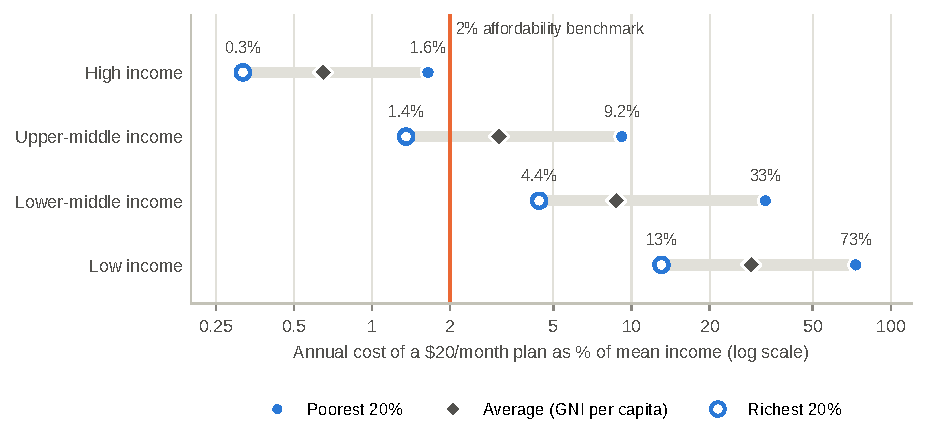
\includegraphics[width=0.92\textwidth]{figures/fig_burden_en.pdf}
\caption{Burden of a \$20 plan across the income distribution. Medians across economies by income group of the annual cost of a \$20/month plan as a share of the mean income of the poorest quintile, of the population (GNI per capita), and of the richest quintile. Quintile incomes are approximated as GNI per capita times the survey income share relative to 20\%. The vertical line marks the 2\% broadband affordability benchmark.}\label{fig:burden}
\end{figure}

Burdens at quintile means give a fuller picture (Figure~\ref{fig:burden}, Table~\ref{tab:quintile}). For the poorest fifth of households, a \$20 plan costs a median 1.6\% of mean income in high-income economies but 33\% in lower-middle- and 73\% in low-income economies. The plan fails the 2\% benchmark even for the richest fifth in every low-income economy with survey data (19) and in 98\% of lower-middle-income economies. In these two groups the median burden for the richest quintile is 13\% and 4.4\%, respectively. Households at the top of the distribution in these economies, where the professionals most likely to use AI at work are concentrated, therefore face burdens several times those of the poorest fifth of households in high-income economies.

\begin{table}[t]
\centering
\begin{threeparttable}
\caption{Burden of a \$20 plan by income quintile, and comparison with mobile broadband (medians)}\label{tab:quintile}
\small
\begin{tabular}{@{}lrrrrrr@{}}
\toprule
 & & \multicolumn{3}{c}{\$20 plan, \% of quintile mean income} & Mobile broadband & AI plan / \\
\cmidrule(lr){3-5}
Income group & $N$ & Poorest 20\% & Middle 20\% & Richest 20\% & 2 GB, \% GNI p.c. & broadband \\
\midrule
\tabinput{tables/tab_quintile.tex}
\bottomrule
\end{tabular}
\begin{tablenotes}[flushleft]\footnotesize
\item \emph{Notes:} Quintile shares from the latest household survey in WDI (median survey year 2021--2023). Mobile broadband: ITU data-only basket with at least 2 GB per month, latest official year (2024), as a share of monthly GNI per capita \citep{itu2025baskets}. The last column is the ratio of the \$20 AI plan's burden to the broadband basket's.
\end{tablenotes}
\end{threeparttable}
\end{table}

\subsection{Local prices: how much do vendors localise?}\label{sec:prices}

Burdens computed at U.S. list prices would overstate the gradient if vendors charged less in poorer markets, but for the most part they do not. Figure~\ref{fig:prices} plots the local App Store price of ChatGPT Plus and ChatGPT Go against per-capita income, and Table~\ref{tab:local} reports, for nine plans, median local prices by income group and the elasticity $\hat\beta$ from regressing log dollar price on log income.

\begin{figure}[t]
\centering
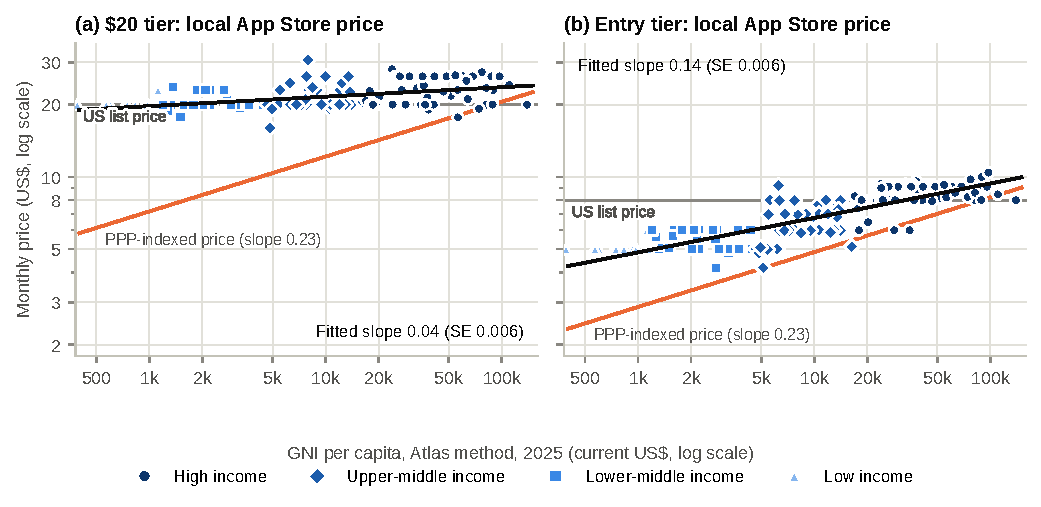
\includegraphics[width=\textwidth]{figures/fig_prices_en.pdf}
\caption{Local App Store prices of ChatGPT Plus and ChatGPT Go against income. Tax-inclusive monthly prices in each national App Store storefront, converted to dollars at market exchange rates on 27 September 2026. Black lines: fitted log-log regressions. Orange lines: prices indexed to local price levels, anchored at the U.S. price, with the slope (0.23) on income of the Atlas-to-PPP income ratio, a price-level proxy. Grey lines: U.S. list prices.}\label{fig:prices}
\end{figure}

\begin{table}[t]
\centering
\begin{threeparttable}
\caption{Local prices and localisation elasticities by plan}\label{tab:local}
\small
\begin{tabular}{@{}lrrrrrrrr@{}}
\toprule
 & U.S. & \multicolumn{4}{c}{Median local price (US\$)} & \multicolumn{2}{c}{Localisation} & \\
\cmidrule(lr){3-6}\cmidrule(lr){7-8}
Plan & price & High & Upper-mid. & Lower-mid. & Low & $\hat\beta$ & (s.e.) & $N$ \\
\midrule
\tabinput{tables/tab_local.tex}
\bottomrule
\end{tabular}
\begin{tablenotes}[flushleft]\footnotesize
\item \emph{Notes:} Monthly App Store prices, 27 September 2026, tax-inclusive except in the U.S. and Canada. $\hat\beta$: OLS slope of $\ln$(local dollar price) on $\ln$(GNI per capita), heteroskedasticity-robust (HC3) standard errors. For reference, the slope on log income of the log price-level proxy (Atlas over PPP GNI) is 0.228 (s.e.\ 0.014), and that of the GDP price-level ratio 0.224. Proportional pricing would imply a slope of 1.
\end{tablenotes}
\end{threeparttable}
\end{table}

The standard and high-usage tiers are priced almost uniformly. For ChatGPT Plus, $\hat\beta = 0.039$ (s.e.\ 0.006), and the estimates for Claude Pro and Google AI Pro are 0.026 and 0.037. The median local price of ChatGPT Plus is \$19.99 in upper-middle-, lower-middle- and low-income storefronts alike, and it is higher, at \$22.99, in the median high-income storefront. Because App Store prices include value-added taxes outside the United States and Canada, the small positive elasticities may reflect taxes rather than price discrimination. Only OpenAI's entry tier is localised to a meaningful degree: ChatGPT Go has $\hat\beta = 0.143$, with median prices of \$9.05, \$5.99, \$5.34 and \$4.99 across the four groups, and lows of \$4.16 in India and \$4.19 in Indonesia. This slope is still only about 63\% of the one implied by indexing to local price levels (0.23), and one-seventh of proportional pricing. Google's entry tier, AI Plus, is flat at \$4.99.

With $\beta$ near zero, the burden elasticity $\beta - 1$ is $-0.96$ for the standard tier: local pricing passes essentially the whole income gradient through to burdens. As Table~\ref{tab:store} shows, every storefront in a low-income economy, and 86\% of those in lower-middle-income economies, prices in U.S. dollars. In 36\% of low-income and 21\% of lower-middle-income economies there is no local storefront at all, so residents must pay through a foreign account or on the web, typically with an international card. The cheapest paid tier listed locally costs \$4.99 in the median low-income economy, a burden of 7.2\%, and it meets the benchmark nowhere in that group. In lower-middle-income economies it does so in 38\% of cases.

\begin{table}[t]
\centering
\begin{threeparttable}
\caption{Storefront availability, currency and the cheapest locally listed paid tier}\label{tab:store}
\footnotesize
\setlength{\tabcolsep}{3pt}
\begin{tabular}{@{}lrrrrrrrr@{}}
\toprule
 & & \multicolumn{3}{c}{ChatGPT storefront (\% of econ.)} & USD & \multicolumn{2}{c}{Cheapest paid tier} & Plus \\
\cmidrule(lr){3-5}\cmidrule(lr){7-8}
Income group & $N$ & Local & None & Not offered & priced (\%) & US\$ & Burden & burden \\
\midrule
\tabinput{tables/tab_store.tex}
\bottomrule
\end{tabular}
\begin{tablenotes}[flushleft]\footnotesize
\item \emph{Notes:} ``No store'': Apple redirects the storefront code to the U.S. store. ``Not offered'': the app is unavailable in the local store. Cheapest paid tier: the lower of ChatGPT Go and Google AI Plus in local storefronts. Burdens are medians of $12p/y\times100$ at local prices.
\end{tablenotes}
\end{threeparttable}
\end{table}

The pattern is consistent with the logic of menu design. Localising the \$20 tier invites arbitrage by high-valuation users through foreign accounts, whereas localising a capability-limited entry tier does not, because high-valuation users self-select into the higher tier \citep{mussa1978monopoly}. Where vendors price-discriminate across countries, they sell degraded quality cheaply but barely localise the prices of frontier tiers. By Proposition~\ref{prop:margins}, price should matter most on the frontier margin, which remains unlocalised.

\subsection{The extensive margin: who uses AI at all}\label{sec:extensive}

Median AI user shares in the second quarter of 2026 were 32.3\% in high-income, 18.8\% in upper-middle-, 12.0\% in lower-middle- and 7.6\% in low-income economies with country-specific estimates (Figure~\ref{fig:dynamics}a). Table~\ref{tab:diffusion} reports the cross-country gradient. On country-specific estimates, a one-log-point increase in income is associated with 8.3 percentage points higher use, and the elasticity is 0.370 (s.e.\ 0.021; $R^2 = 0.71$). Including pooled regional values lowers the elasticity to 0.336; collapsing each pool to one observation restores it (0.367). The elasticity is unchanged by controls for internet use, tertiary enrolment, urbanisation, age structure, digital payments and region fixed effects (0.357--0.367). Conditional on income, none of the controls is individually significant except urbanisation in columns (3)--(4) ($p \approx 0.04$), which loses significance once region fixed effects are added (Appendix Table~\ref{tab:controls}).

\begin{table}[t]
\centering
\begin{threeparttable}
\caption{Income gradient of generative-AI use (Microsoft AI User Share, Q2 2026)}\label{tab:diffusion}
\small
\setlength{\tabcolsep}{5pt}
\begin{tabular}{@{}lrrrrrrr@{}}
\toprule
 & (1) & (2) & (3) & (4) & (5) & (6) & (7) \\
 & Level (pp) & \multicolumn{6}{c}{Log user share} \\
\cmidrule(lr){3-8}
\midrule
\tabinput{tables/tab_diffusion.tex}
\bottomrule
\end{tabular}
\begin{tablenotes}[flushleft]\footnotesize
\item \emph{Notes:} OLS with HC3 standard errors in parentheses. CS: country-specific estimates only; All: including region-imputed values; Coll.: each region-imputed pool collapsed to one observation with population-weighted log income. $^\dagger$Common sample with non-missing controls (internet use, tertiary enrolment, urban share, population 65+, share making digital online merchant payments). Coefficients on controls in Appendix Table~\ref{tab:controls}.
\end{tablenotes}
\end{threeparttable}
\end{table}

\paragraph{Half of the gradient mirrors connectivity.} Because use requires connection, the user share can be written as $D_c = I_c \times (D_c/I_c)$, the product of the internet-use rate and the ratio of AI users to internet users, which I call adoption among internet users. The ratio is an accounting construct, not an observed conditional adoption rate. Regressing each log component on log income decomposes the elasticity exactly: connectivity contributes 0.182 and adoption among the connected 0.189, so the connectivity component accounts for 49\% of the gradient. The split is an accounting identity rather than a causal share: holding income fixed, the elasticity of AI use with respect to internet use is 0.05 (s.e.\ 0.20), far from the value of one that a pure connectivity channel would imply, and Microsoft's estimator itself adjusts for internet penetration. Across groups (Table~\ref{tab:decomp}, Figure~\ref{fig:decomp}) the connectivity share of the gap to high-income economies rises from 21\% for upper-middle-income to 49\% for lower-middle-income and 67\% for the three low-income economies with country-specific data. Adoption among internet users is flat below the high-income group, at 22.7\%, 23.6\% and 23.0\% from the upper-middle- to the low-income group, against 37.5\% in high-income economies. Its slope on log income across non-high-income economies is $-0.03$ (s.e.\ 0.06), even though the burden of a paid plan rises more than ninefold across those three groups. The comparison rests on group means (the low-income mean covers three economies) and mixes age bases. Still, other things equal, a binding price constraint on the extensive margin would tend to make adoption among the connected fall as the burden rises. Across the three groups it does not, although other differences between the groups could offset such an effect. The gap below high income coincides with connection, and the gap to high income with something that distinguishes high-income economies as a group (workplace integration, desktop use, language). Proposition~\ref{prop:margins} implies that price does not enter the extensive margin when a free tier exists, but the flatness itself is not implied by the model and may partly reflect measurement. The pattern echoes Microsoft's own finding that connected populations in low-penetration economies adopt at rates comparable to the global average \citep{misra2025measuring}.

\begin{table}[t]
\centering
\begin{threeparttable}
\caption{Connectivity decomposition of the AI-use gap (country-specific estimates, Q2 2026)}\label{tab:decomp}
\small
\setlength{\tabcolsep}{4.5pt}
\begin{tabular}{@{}lrrrrrrrr@{}}
\toprule
 & & \multicolumn{3}{c}{Group means (\%)} & \multicolumn{3}{c}{Log gap to high income} & Connectivity \\
\cmidrule(lr){3-5}\cmidrule(lr){6-8}
Income group & $N$ & AI users & Internet & AI $|$ online & Total & Connect. & Adoption & share (\%) \\
\midrule
\tabinput{tables/tab_decomp.tex}
\bottomrule
\end{tabular}
\begin{tablenotes}[flushleft]\footnotesize
\item \emph{Notes:} $\ln D = \ln I + \ln(D/I)$ with $D$ the AI user share (population 15--64) and $I$ internet users (\% of population, latest year). Log gaps are differences between group means of log values (log ratios of geometric means), so they differ from log ratios of the arithmetic means shown. The low-income row rests on three economies and is indicative only. The ratio $D/I$ mixes age bases and is capped at one.
\end{tablenotes}
\end{threeparttable}
\end{table}

\begin{figure}[t]
\centering
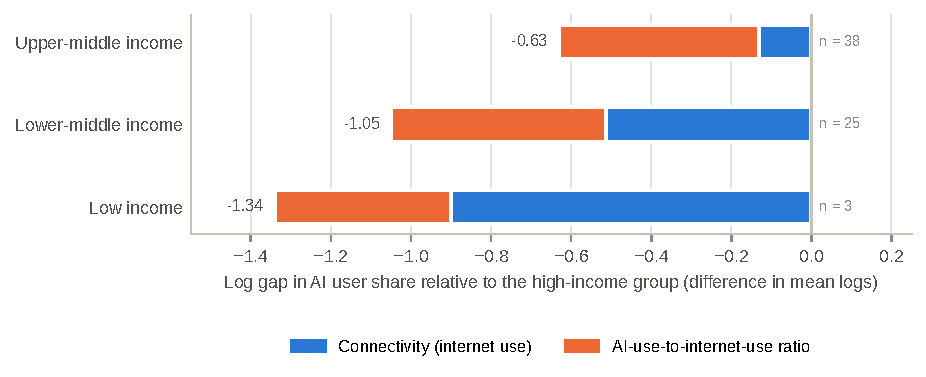
\includegraphics[width=0.9\textwidth]{figures/fig_decomp_en.pdf}
\caption{Decomposition of the log gap in AI use relative to the high-income group (difference in group means of log shares) into connectivity (internet use) and adoption among internet users. Country-specific Microsoft estimates, Q2 2026; the low-income bar rests on three economies.}\label{fig:decomp}
\end{figure}

\paragraph{Relative convergence, absolute divergence.} Between the first half of 2025 and the second quarter of 2026 the median economy's user share rose by 5.5 points in the high-income group, 3.7 in the upper-middle-, 2.0 in the lower-middle- and 0.9 in the low-income group (Figure~\ref{fig:dynamics}). Proportional growth was similar in the three higher groups (21--26\%), and lagging economies grew slightly faster in logs: regressing log growth on the initial log share gives $-0.026$ (s.e.\ 0.011), and the cross-country standard deviation of log shares fell from 0.564 to 0.553. In percentage points the opposite holds: each log point of income is associated with a 1.37-point larger gain (s.e.\ 0.13), the standard deviation rose from 10.9 to 12.8 points, and the gap between the median high- and lower-middle-income economy widened from 16.3 to 20.3 points. This reconciles apparently conflicting reports of faster growth in lower-income countries \citep{chatterji2025how} and of a widening divide \citep{microsoft2026h2,liu2025who}, which are consistent with two readings of an early-phase S-curve.

\begin{figure}[t]
\centering
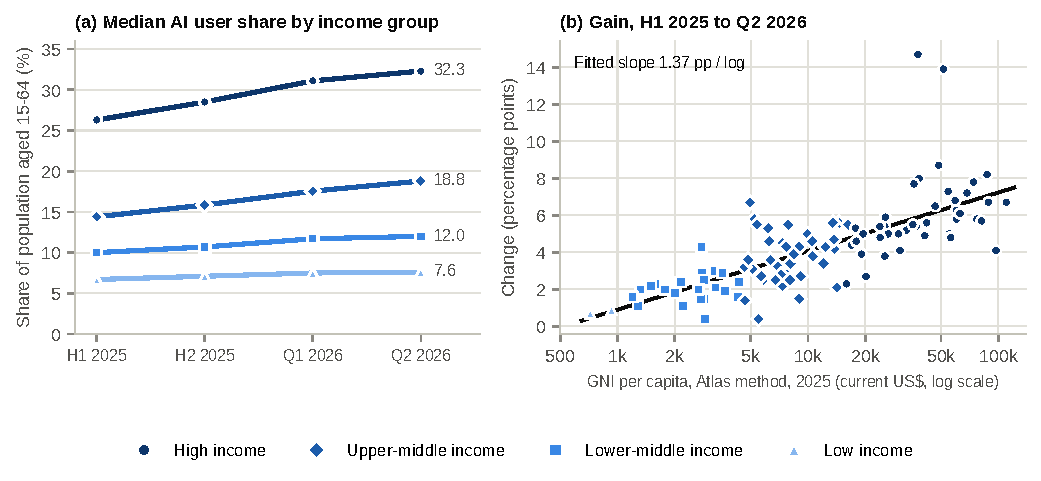
\includegraphics[width=\textwidth]{figures/fig_dynamics_en.pdf}
\caption{Diffusion dynamics. (a) Median AI user share by income group, country-specific Microsoft estimates (low-income: three economies). (b) Change in the AI user share between H1 2025 and Q2 2026 against GNI per capita, with the fitted log-linear slope.}\label{fig:dynamics}
\end{figure}

\subsection{The frontier margin: how much frontier AI is used}\label{sec:twomargins}

Figure~\ref{fig:twomargins} plots both measures, as log deviations from their cross-country means, against income for the 96 economies covered by both: 42 high-, 33 upper-middle-, 20 lower-middle- and one low-income economy (Rwanda). The comparison therefore describes the gradient from lower-middle to high income and says little about low-income economies. The frontier-use index rises twice as steeply: its income elasticity is 0.711 (s.e.\ 0.036) against 0.371 (s.e.\ 0.026) for any use, a difference of 0.340 (clustered s.e.\ 0.034; bootstrap 95\% interval 0.27--0.40). Table~\ref{tab:twomargins} shows that the gap is not an artefact of functional form or sample. It persists when the user share is expressed in log-odds to allow for ceiling effects (0.50 versus 0.71), when high-income economies are excluded (0.33 versus 0.69), conditional on internet use, tertiary enrolment and urbanisation (0.31 versus 0.55), in earlier measurement windows (0.38 versus 0.62), and when pooled regional values are included (0.36 versus 0.73).

\begin{figure}[t]
\centering
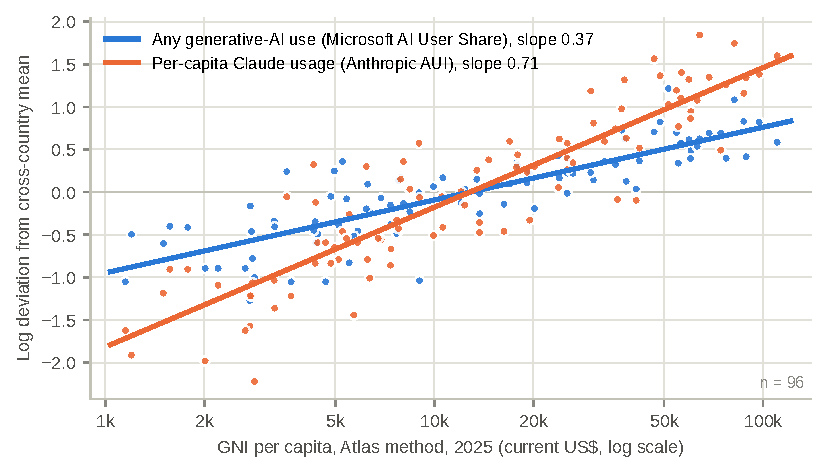
\includegraphics[width=0.9\textwidth]{figures/fig_two_margins_en.pdf}
\caption{Two margins of AI diffusion. Log deviation from the cross-country mean of the Microsoft AI User Share (any generative-AI use, Q2 2026, country-specific estimates) and of the Anthropic AI Usage Index (per-capita Claude use, May 2026) against GNI per capita, for the 96 economies covered by both. Lines are OLS fits; slopes are income elasticities.}\label{fig:twomargins}
\end{figure}

\begin{table}[t]
\centering
\begin{threeparttable}
\caption{Income elasticities on the extensive and frontier margins}\label{tab:twomargins}
\small
\begin{tabular}{@{}>{\raggedright\arraybackslash}p{7.6cm}ccr@{}}
\toprule
Specification & Any use (MS) & Frontier use (AUI) & $N$ \\
\midrule
\tabinput{tables/tab_twomargins.tex}
\bottomrule
\end{tabular}
\begin{tablenotes}[flushleft]\footnotesize
\item \emph{Notes:} Each cell is the OLS slope of the log outcome on log GNI per capita (HC3 standard errors in parentheses) in a common sample. MS: Microsoft AI User Share; AUI: Anthropic AI Usage Index. The difference test stacks both outcomes with an outcome-specific intercept and slope, clustering by economy. The bootstrap resamples economies 2,000 times. The main sample comprises 42 high-, 33 upper-middle-, 20 lower-middle- and one low-income economy. Excluding high-income economies leaves 54.
\end{tablenotes}
\end{threeparttable}
\end{table}

The measured frontier gradient also steepened, though not continuously. On the 111 economies observed in all five windows, the elasticity was 0.68 in August and November 2025, 0.74 in February 2026, 0.77 in April and 0.73 in May 2026. The increase from August 2025 to February 2026 (0.064, clustered s.e.\ 0.018) is significant, whereas the change from February to May 2026 is not ($-0.006$, s.e.\ 0.016). Anthropic's releases changed over this period, adding Max accounts by February 2026 and, from April 2026, Cowork sessions and monthly windows, so the comparison describes the gradient of measured Claude use rather than a strictly like-for-like series. Estimates on all economies meeting Anthropic's thresholds in each window are similar (Appendix Table~\ref{tab:auitime}). The steepening is in line with Anthropic's own finding that low-adoption countries fell slightly further behind \citep{massenkoff2026learning}. The composition of use differs as well: the share of Claude conversations devoted to coursework falls by 4.7 points per log point of income, from 35\% in the median low-income economy (five economies) to 17\% in the median high-income economy. This gradient is consistent with evidence that learning is a leading entry point in lower-income regions \citep{microsoft2026q2,daepp2026how} and with Anthropic's observation that coursework may be better suited to free use \citep{appel2026primitives}. A third source, Google's per-capita adoption quintile for Gemini, is also positively but less tightly related to income (Spearman correlation 0.46 across 195 economies), which may reflect Gemini's distribution through Android and Search at zero price.

These patterns are consistent with Proposition~\ref{prop:margins} when the paid hurdle exceeds the free hurdle and localisation is weak ($\hat\beta \approx 0.04$ at the \$20 tier). They do not establish that prices cause the steeper frontier gradient. Section~\ref{sec:discussion} discusses alternative explanations.

\subsection{Illustrative aggregate implications}\label{sec:scenarios}

Table~\ref{tab:scen} and Figure~\ref{fig:scen} apply the Hulten-style formula of equation~\eqref{eq:ratio} with proxy inputs and task-level gains of 10--30\%, bracketing the 15\% of \citet{brynjolfsson2025generative} and the 26\% increase in completed tasks of \citet{cui2024effects}. Exposure $E$ is proxied by the share of employment in occupations exposed to generative AI \citep{gmyrek2025generative} and adoption $a$ by the share of the working-age population that uses any generative-AI product. Neither matches the formula's definitions: occupational exposure overstates the share of tasks exposed when only some tasks of an exposed occupation are affected, and population-wide use understates adoption in exposed tasks if users concentrate in exposed jobs but overstates it if their use is occasional. The results are therefore orders of magnitude, not estimates. With a labour share of 0.55 and a 20\% task-level gain, the illustrative gains are 1.21\% of GDP in high-income economies, 0.48\% in upper-middle-, 0.21\% in lower-middle- and 0.11\% in low-income economies. These levels are five to seventeen times smaller than the naive product of adoption and task-level gains used in the earlier draft (6.5\% and 1.8\% for the first and last groups), which ignores that AI touches only exposed tasks and that labour is only part of value added. The magnitudes are in line with \citet{acemoglu2025simple}. The ratio between high- and low-income economies is eleven-fold (thirteen-fold if low-income adoption is measured by the three country-specific estimates) and reflects exposure and adoption jointly: even at high-income adoption rates, low-income gains would rise only to 0.39\%.

\begin{table}[t]
\centering
\begin{threeparttable}
\caption{Illustrative output gains from generative AI (\% of GDP)}\label{tab:scen}
\footnotesize
\setlength{\tabcolsep}{4pt}
\begin{tabular}{@{}lrrrrrrr@{}}
\toprule
 & Exposed & Adoption & Naive $a\cdot g$ & \multicolumn{3}{c}{Hulten: $s_L E a g$} & At high-income \\
\cmidrule(lr){5-7}
Income group & $E$ (\%) & $a$ (\%) & $g=20\%$ & $g=10\%$ & $g=20\%$ & $g=30\%$ & adoption, $g=20\%$ \\
\midrule
\tabinput{tables/tab_scen.tex}
\bottomrule
\end{tabular}
\begin{tablenotes}[flushleft]\footnotesize
\item \emph{Notes:} $s_L = 0.55$. Exposure: share of employment in occupations exposed to generative AI, 34\% in high- and 11\% in low-income economies \citep{gmyrek2025generative}; middle groups are geometric interpolations. Adoption: median Microsoft AI User Share in Q2 2026 (low-income: all economies, including pooled values). Illustrations, not forecasts: they ignore reallocation, prices, capital deepening and new tasks. Expressing task-level gains as cost savings, $g/(1+g)$, would lower all figures by about a sixth.
\end{tablenotes}
\end{threeparttable}
\end{table}

\begin{figure}[t]
\centering
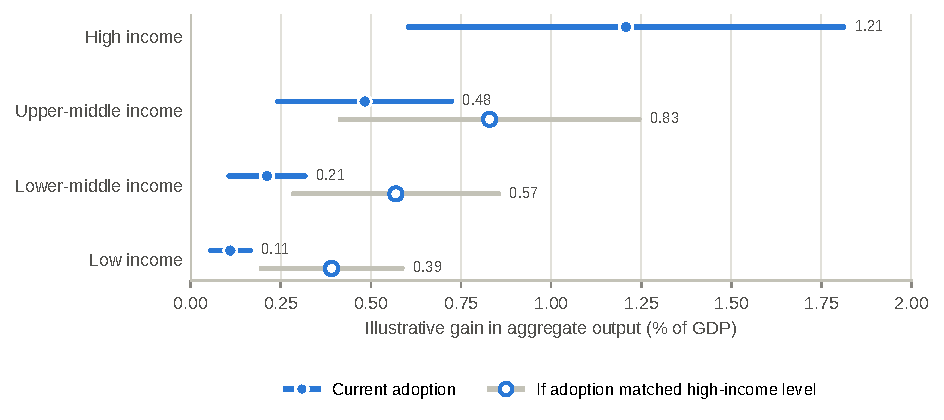
\includegraphics[width=0.9\textwidth]{figures/fig_scen_en.pdf}
\caption{Illustrative output gains. Hulten-style gains $s_L E a g$ with $s_L=0.55$ and proxy inputs: occupational exposure from \citet{gmyrek2025generative} and population-wide AI use at current (filled markers) or high-income levels (hollow markers). Bars span task-level gains of 10--30\%; markers and labels show 20\%.}\label{fig:scen}
\end{figure}

Proposition~\ref{prop:equal} makes the equalisation arithmetic explicit. On the same proxies, with $E_H/E_L = 34/11$ and $a_H = 0.32$, avoiding divergence would require low-income adoption of $a_L^* = 1.00$ if task-level gains were equal, 0.67 if they were 1.5 times larger in low-income economies, and 0.50 if twice as large, compared with roughly 0.09 today. On these numbers the AI access paradox is large: at the task-level gains illustrated here, differences in exposure and access swamp conditional equalisation.

% ================================================================================================
\section{Discussion}\label{sec:discussion}

\subsection{What the evidence does and does not show}

The evidence supports three statements. Identical dollar prices impose burdens that differ by a factor of about 45 across income groups, and the only material localisation is of a degraded entry tier. The extensive margin of AI use is moderately income-graded: about half of the gradient mirrors the gradient in internet use, and in these cross-country data adoption among the connected does not decline with the burden of a paid plan, although an independent price effect is not tested. The frontier margin, as proxied by per-capita Claude use, is about twice as income-graded, and its measured gradient rose between late 2025 and early 2026.

The evidence does not establish that prices cause the steeper frontier gradient. Several alternatives could contribute. \emph{Language}: frontier assistants perform best in high-resource languages, and English-language interactions are over-represented where local languages are poorly supported \citep{daepp2026how}. \emph{Product and brand}: Claude is less known in many lower-income markets than ChatGPT, Gemini or Meta's assistant. \emph{Work composition}: Claude's usage skews toward software and professional tasks, whose share of employment rises with income \citep{gmyrek2025generative}. \emph{Measurement}: Microsoft's estimator shrinks noisy countries toward the global average and floors device-scaling factors, which compresses cross-country variation and may flatten the measured extensive gradient \citep{misra2025measuring}. The robustness checks address some of these concerns (the gap persists without high-income economies and conditional on education), but the only credible route to a price effect is variation in prices that is not a function of income.

Such variation now exists. ChatGPT Go was rolled out to India and then to 170 further countries on a staggered schedule \citep{openai2026go}; Google introduced and repriced AI Plus and AI Ultra in 2025--2026 \citep{google2026io}; several markets saw temporary free premium tiers bundled with mobile subscriptions; and App Store price schedules change with exchange rates and taxes. Combined with the quarterly Microsoft series and the monthly Anthropic series, these events support difference-in-differences and event-study designs that compare economies before and after a localised tier becomes available, with the frontier margin as the outcome of interest. Vendors could make such evaluations far more precise by publishing country-level paid-subscription counts and effective prices.

\subsection{Policy implications}

The results suggest four priorities, ordered by the margin they address.

\emph{Connectivity as a precondition, for the extensive margin.} Connection, devices and electricity are preconditions for any use, and half of the use gradient mirrors the connectivity gradient. The cross-country data cannot isolate the marginal effect of connectivity on AI use. The flat adoption rate among the connected is consistent with the view that access and complements, rather than price, limit whether the connected use AI at all \citep{worldbank2026wdr,itu2025ff}, although it does not demonstrate this. Compute and data infrastructure add a further layer \citep{lehdonvirta2024compute}. Evidence from fast internet in Africa suggests that such investments raise employment and productivity in their own right \citep{hjort2019arrival}.

\emph{Localise frontier access, not only degraded tiers, for the frontier margin.} Welfare effects of third-degree price discrimination are ambiguous in general, but they tend to be positive when discrimination opens markets that uniform pricing would leave unserved \citep{varian1985price,aguirre2010monopoly}, as may be the case for frontier tiers where the list price exceeds a quarter of average income. Local-currency storefronts, carrier billing and time-limited or usage-limited frontier access at locally indexed prices are practical steps. The arbitrage risk that keeps the \$20 tier uniform can be contained with usage caps rather than by withholding frontier models.

\emph{Institutional access.} Evidence on AI's productivity effects comes overwhelmingly from employer-provided tools rather than individual subscriptions \citep{brynjolfsson2025generative,cui2024effects}. Schools, universities, public agencies and employers can decouple access from household income. A World Bank trial in Nigeria, for example, found sizeable learning gains from a supervised GPT-4 tutoring programme \citep{desimone2025chalkboards}. Research on short-run subsidies for new health products suggests that free trials can raise long-run adoption through learning rather than crowding it out \citep{dupas2014short}, while even small prices can sharply reduce take-up among the poor \citep{cohen2010free}.

\emph{Transparency.} Research on AI access is constrained by the absence of public data on paid subscriptions, effective prices and usage limits by country. Machine-readable disclosure of country-level prices, taxes, supported payment methods and plan limits would allow the designs described above to be implemented.

\subsection{Limitations}

First, burdens are normalised prices rather than expenditures, and quintile incomes are approximations based on survey shares that mix income and consumption concepts. Second, App Store prices can differ from web prices and include platform commissions, and the audit is a single-day cross-section that omits promotions and bundles. Third, the Microsoft series is a modelled estimate built on desktop telemetry, and country-specific values are unavailable for most low-income economies. Results for that group rest on three economies or on regional pools, and the two-margin comparison includes a single low-income economy. Fourth, the Anthropic index covers one vendor's consumer product and does not distinguish paid from free users, so it proxies the frontier margin imperfectly. Fifth, all regressions are cross-sectional and descriptive. Sixth, the aggregate illustrations proxy task exposure with occupational exposure and within-task adoption with population-wide use, assume common task-level gains, ignore general-equilibrium effects and use interpolated exposure shares for middle-income groups. They also omit consumer surplus from free use, which measured output misses for digital goods \citep{brynjolfsson2019using} and which may be large where AI is used mainly for learning. Seventh, the capability lag is calibrated on API inference prices, not on the prices of consumer subscription tiers.

% ================================================================================================
\section{Conclusion}\label{sec:conclusion}

Generative AI is priced as a global product and experienced as a local one. The standard \$20 plan is priced almost identically everywhere. It costs less than 1\% of average income in the median rich country and more than a quarter in the median poor one, and it fails the broadband affordability benchmark for most of the world's working-age population and, in low-income economies, even for the richest fifth. The evidence is consistent with free tiers having taken price out of the decision whether to use AI at all. On that margin, about half of the income gradient coincides with the gradient in connectivity. How intensively people use a frontier assistant, by contrast, remains tied to income: in the Claude data its gradient is twice as steep and rose between late 2025 and early 2026. The staggered rollout of localised tiers now makes it possible to test whether price is what ties frontier use to income, rather than language, product reach or the composition of work.

The conditional evidence that AI helps less-experienced workers most is real, but conditional equalisation does not aggregate into convergence unless access and exposure keep pace, and on current numbers they do not. Whether they will depends more on who can access or afford frontier models, for how much use and how soon after release, than on how capable the models become.

% ================================================================================================
\section*{Declarations}
\paragraph{Declaration of generative AI and AI-assisted technologies in the manuscript preparation process.} During the preparation of this work the author used ChatGPT (OpenAI) and Claude (Anthropic) to assist with literature search, coding and data processing, drafting and translation, and GPT-6 Astra (OpenAI) to check the methods and the replication package. After using these tools, the author reviewed and edited the content as needed and takes full responsibility for the content of the publication.
\paragraph{Data availability.} All data are publicly available. The accompanying replication package contains the extracts, code and outputs described in Appendix~\ref{app:data}. It is deposited at Zenodo under DOI \href{https://doi.org/10.5281/zenodo.23006366}{\mbox{10.5281/zenodo.23006366}}.
\paragraph{Funding and competing interests.} The author received no specific funding for this work and declares no competing interests.

\bibliographystyle{plainnat}
\bibliography{references}

% ================================================================================================
\clearpage
\appendix
\section{Proofs}\label{app:proofs}

\paragraph{Proposition~\ref{prop:margins}.} From \eqref{eq:margins}, $\ln D_c = \ln\kappa_c + \ln\Phi(z^D_c)$. Since $\mu_c$ moves one-for-one with log income, $\partial z^D_c/\partial \ln y_c = 1/s$, so $\varepsilon_D = \varepsilon_\kappa + h(z^D_c)/s$. For the frontier margin, $z^P_c = [\mu_c - \ln p_c + \ln(q_P - q_F)]/s$ and $\partial z^P_c/\partial \ln y_c = (1-\beta)/s$, so $\varepsilon_P = \varepsilon_\kappa + (1-\beta)h(z^P_c)/s$. If $p_c/(q_P-q_F) > \tau/q_F$ then $z^P_c < z^D_c$, and because the inverse Mills ratio $h$ is strictly decreasing, $h(z^P_c) > h(z^D_c)$; with $\beta = 0$ this gives $\varepsilon_P > \varepsilon_D$. The difference $\varepsilon_P - \varepsilon_D = [(1-\beta)h(z^P_c) - h(z^D_c)]/s$ is decreasing in $\beta$ (holding $z$'s fixed) and equals $-h(z^D_c)/s < 0$ at $\beta = 1$, so it changes sign at $\beta^* = 1 - h(z^D_c)/h(z^P_c) \in (0,1)$. \qed

\paragraph{Proposition~\ref{prop:equal}.} From \eqref{eq:ratio}, $R_1 < R_0$ iff $1 + s_LE_Ha_Hg_H < 1 + s_LE_La_Lg_L$, i.e.\ iff $E_La_Lg_L > E_Ha_Hg_H$. Solving the equality for $a_L$ gives $a_L^*$. If $g_L > g_H$ but $a_L E_L < a_H E_H g_H/g_L$, the gap widens, so $g_L > g_H$ is not sufficient; if $g_L \le g_H$ but $a_L E_L$ is large enough, the gap narrows, so it is not necessary. \qed

\paragraph{Proposition~\ref{prop:lag}.} The capability that was at the frontier at $t-L$ costs $\bar p e^{-\delta L}$ at $t$; setting this equal to $b$ gives $L = \ln(\bar p/b)/\delta$. With $\delta \in [\ln 9, \ln 900] = [2.20, 6.80]$ per year and budgets equal to 2\% of median monthly GNI per capita (\$1.38 in low-income and \$4.58 in lower-middle-income economies), $L \in [0.39, 1.22]$ and $[0.22, 0.67]$ years, respectively. \qed

% ------------------------------------------------------------------------------------------------
\section{Data construction and replication}\label{app:data}

\paragraph{Replication package.} The package contains the World Bank API extracts, the Microsoft dataset at commit 507c316, Google ATLAS data, the App Store and exchange-rate snapshots, and derived country-level files for the Anthropic Economic Index and ITU price baskets. The original Anthropic release files and ITU workbook are not bundled; the download script retrieves the sources documented in the README so that these country-level files can also be rebuilt. The package also contains the processing scripts (\nolinkurl{01_download_wb.py}, \nolinkurl{02_scrape_appstore_prices.py}, \nolinkurl{09_appstore_prices.py}, \nolinkurl{10_build_dataset.py}), the analysis (\nolinkurl{20_analysis.py}), figures (\nolinkurl{30_figures.py}) and table generation (\nolinkurl{40_tables_tex.py}). Every number in the text can be reproduced from the package. Most are written to \nolinkurl{output/results.json}. The rest are simple calculations from those values, such as ratios and the capability-lag calibration, or are read from the output tables, the processed data or the scripts. The README follows the template of the Social Science Data Editors.

\paragraph{App Store audit.} Requests were made on 27 September 2026 (UTC) to \nolinkurl{https://apps.apple.com/<cc>/app/id<app>} for ChatGPT (6448311069), Claude (6473753684) and Google Gemini (6477489729), using the two-letter codes of all 217 World Bank economies plus Taiwan. Of 654 requests, 500 returned local pages, 135 were redirected to the U.S. store and 19 returned ``not found''. Prices were parsed from the displayed strings, including locale-specific separators and abbreviations (e.g.\ Indonesian ``ribu'' and ``juta''). Four storefront-plan cells in which the observed page listed only an annual price were dropped. In three cells two different monthly prices are listed for the same plan: Google AI Pro in India and T\"urkiye, where one of five listings carries a lower price, and in Benin, where a 10 TB variant is listed alongside the standard plan. I use the modal price. Taking the lowest listed price instead changes the Google AI Pro elasticity by 0.0001.

\paragraph{Microsoft region-imputed economies.} Six pools with identical four-period series: West Africa (Benin, Burkina Faso, Ghana, Guinea, Guinea-Bissau, Liberia, Mali, Mauritania, Niger, Nigeria, Sierra Leone, Togo); East Africa (Burundi, Eritrea, Ethiopia, Somalia, South Sudan, Sudan, Tanzania, Uganda); Central Africa (Cameroon, Central African Republic, Chad, Congo, Congo DR); Southern Africa (Angola, Madagascar, Malawi, Mozambique); the Guianas (French Guiana, Guyana, Suriname) and Venezuela; and Afghanistan, Tajikistan and Turkmenistan. These 36 economies coincide with those marked as region-imputed in \citet[Appendix Table 2]{misra2025measuring}. Because French Guiana and Taiwan are not World Bank economies, 145 Microsoft economies are matched and 142 have income data.

\paragraph{Anthropic index.} Published AUIs are used for April and May 2026. For August and November 2025 and February 2026 the index is recomputed as usage share over working-age population share among geolocated countries with at least 200 sampled conversations, because the August 2025 published values include un-geolocated traffic in the usage denominator (scaling all values by a common factor of 0.843) and later releases publish counts rather than indices.

% ------------------------------------------------------------------------------------------------
\section{The earlier 24-country design revisited}\label{app:orig}

The earlier draft analysed a purposive sample of 24 economies with 2022 incomes. Table~\ref{tab:case} updates that sample. The update brings three corrections. (i) Seven of the 24 diffusion values (Nigeria, Ghana, Niger, Uganda, Malawi, Mozambique and Madagascar, including five of the six low-income economies in the sample) are regional averages, so the earlier finding that low-income and lower-middle-income user shares were similar (10.0\% versus 11.4\%) partly reflects imputation. Among country-specific values the low-income group contains only Rwanda (7.6\%). (ii) Current World Development Indicators revise several 2022 incomes. With the revised values, the correlation between log income and the user share in the 24-economy sample is 0.827 (0.839 among the 17 country-specific values). (iii) Local App Store listings differ from U.S. prices: in Kenya, Ghana and Uganda, ChatGPT Plus is listed at \$22.99, above the \$19.99 U.S. listing. Bangladesh has no local storefront, and ChatGPT is not offered in China.

\begin{table}[ht]
\centering
\begin{threeparttable}
\caption{The 24 case economies with updated data}\label{tab:case}
\scriptsize
\setlength{\tabcolsep}{3.5pt}
\begin{tabular}{@{}llrrrrrlrr@{}}
\toprule
Economy & Group & GNI p.c. 2025 & Burden \$20 & Plus (US\$) & Burden Plus & Go (US\$) & Currency & AI users (\%) & AUI \\
\midrule
\tabinput{tables/tab_case.tex}
\bottomrule
\end{tabular}
\begin{tablenotes}[flushleft]\footnotesize
\item \emph{Notes:} Burdens in \% of GNI per capita. Plus and Go: local App Store prices. AI users: Microsoft AI User Share, Q2 2026; $^\ddagger$region-imputed. AUI: Anthropic AI Usage Index, May 2026 (-- = not published).
\end{tablenotes}
\end{threeparttable}
\end{table}

\clearpage % keep the Appendix C table ahead of Appendix D
% ------------------------------------------------------------------------------------------------
\section{Additional tables}\label{app:tables}

\begin{table}[ht]
\centering
\begin{threeparttable}
\caption{Income gradient of AI use with controls (log user share, country-specific, common sample)}\label{tab:controls}
\small
\begin{tabular}{@{}lrrrrr@{}}
\toprule
 & (1) & (2) & (3) & (4) & (5) \\
\midrule
\tabinput{tables/tab_controls.tex}
\bottomrule
\end{tabular}
\begin{tablenotes}[flushleft]\footnotesize
\item \emph{Notes:} OLS with HC3 standard errors. Controls measured in percent; Findex 2025 for digital payments.
\end{tablenotes}
\end{threeparttable}
\end{table}

\begin{table}[ht]
\centering
\begin{threeparttable}
\caption{Income elasticity of the Anthropic AI Usage Index over time}\label{tab:auitime}
\small
\begin{tabular}{@{}lrrrrrr@{}}
\toprule
 & \multicolumn{4}{c}{All qualifying economies} & \multicolumn{2}{c}{Common sample ($N=111$)} \\
\cmidrule(lr){2-5}\cmidrule(lr){6-7}
Window & Elasticity & (s.e.) & $N$ & $R^2$ & Elasticity & (s.e.) \\
\midrule
\tabinput{tables/tab_aui_time.tex}
\bottomrule
\end{tabular}
\begin{tablenotes}[flushleft]\footnotesize
\item \emph{Notes:} OLS of log AUI on log GNI per capita (2025); economies with at least 200 sampled conversations (Aug 2025--Feb 2026) or with published values (Apr--May 2026). Common sample: economies qualifying in all five windows; change Aug 2025 to Feb 2026: 0.064 (clustered s.e.\ 0.018); Feb to May 2026: $-0.006$ (0.016).
\end{tablenotes}
\end{threeparttable}
\end{table}

\end{document}
